\documentclass{article}
\usepackage[a4paper, left=15mm, top=20mm, right=15mm,bottom=20mm]{geometry}
\usepackage{amsmath, amssymb, amsfonts}
\usepackage{fancyhdr}
\usepackage{graphicx}
\graphicspath{ {./images/} }
\usepackage{float}
\usepackage{hyperref}
\usepackage{lscape}
\usepackage{multirow}

\pagestyle{fancy}
\fancyhf{}
\lhead{ACC1701X}
\rhead{claudeonrs}
\rfoot{\thepage}
\usepackage{amsmath, amssymb, amsfonts, listings}
\usepackage{xcolor}
\usepackage{enumitem}
\setlist[itemize]{noitemsep, topsep=0pt}
\setlist[enumerate]{noitemsep, topsep=0pt}
\setlist[description]{noitemsep, topsep=0pt}


%New colors defined below
\definecolor{codegreen}{rgb}{0,0.6,0.4}
\definecolor{codegray}{rgb}{0.5,0.5,0.5}
\definecolor{codepurple}{rgb}{0.58,0,0.82}
\definecolor{backcolour}{rgb}{0.95,0.95,0.92}
\definecolor{commentgreen}{rgb}{0.4,0.8,0.6}
%Code listing style named "mystyle"
\lstdefinestyle{mystyle}{
  backgroundcolor=\color{backcolour},
  commentstyle=\color{red},
  keywordstyle=\color{blue},
  numberstyle=\tiny\color{codegray},
  stringstyle=\color{codegreen},
  basicstyle=\ttfamily,
  breakatwhitespace=false,
  breaklines=true,
  captionpos=b,
  keepspaces=true,
  numbers=left,
  numbersep=5pt,
  showspaces=false,
  showstringspaces=false,
  showtabs=false,
  tabsize=2
}

%"mystyle" code listing set
\lstset{style=mystyle}

\title{No Title}
\author{Claudeon R Susanto}
\date{}
\usepackage[T1]{fontenc}
\usepackage[utf8]{inputenc}
\usepackage[english]{babel}
\usepackage{lmodern}

\renewcommand{\familydefault}{\sfdefault}   % Supprime le serif (dyslexie)
\usepackage[font=sf, labelfont={sf}]{caption}
\usepackage{multicol}
\usepackage{makecell}
\renewcommand\theadalign{bc}
\renewcommand\theadfont{\bfseries}
\renewcommand\theadgape{\Gape[4pt]}
\renewcommand\cellgape{\Gape[4pt]}



% own commands
\newcommand{\eg}[0]{\textit{e.g. }}
\newcommand{\ie}[0]{\textit{i.e. }}
\newcommand{\impt}[0]{\textcolor{red}{\textbf{[IMPT] }}}


\renewcommand\thesubsection{\thesection.\arabic{subsection}}
\setlength{\columnseprule}{1pt}
\begin{document}
%\maketitle
\fontfamily{lmss}\selectfont
\begin{multicols}{2}
\section{Accounting in Business}
\begin{description}
	\item[in the aggregate] accumulate transactions of the same type over a certain period and report the data as one amount in the company's financial statements
	\item[accounting] the entire process of identifying, recording, and communicating economic events (bookkeeping is part of recording only)\\
\end{description}
\textbf{Who uses accounting data?}
\begin{itemize}[topsep=0pt]
	\item \textbf{Internal users}\\
	\underline{Managerial accounting} provides internal reports to help users make decisions about their companies
	\begin{itemize}
		\item Management
		\item Employees
	\end{itemize}
	\item \textbf{External users} (investors and creditors, etc.)\\
	\underline{Financial accounting} provides economic and financial information for investors, creditors, and other external users
	\begin{itemize}
		\item Lenders
		\item Investors
		\item Competitors
		\item Government agencies\\
		IRS:
		SEC:
		\item The press
	\end{itemize}
\end{itemize}
\textbf{Measurement principles} (used by IFRS)
\begin{itemize}
	\item \impt Follow trade-offs between \textbf{relevance} (makes a difference in decision making) and \textbf{faithful representation} (factual and accurate)
	\item \impt Enhancing qualitative characteristics (\textbf{Comparability, Verifiability, Timeliness, Understandability})
	\item \textbf{Historical cost} principle: record assets at their initial cost when it was purchased
	\item \textbf{Fair value} principle: assets and liabilities should be reported at fair value (\underline{price received to sell an asset or settle a liability})
	\begin{itemize}
		\item Only used when asses are actively traded, otherwise rarely used
		\item Also used when market value info is available for certain assets\\
	\end{itemize}
\end{itemize}
\textbf{Accounting assumptions}
\begin{itemize}
	\item \textbf{Monetary unit} assumption: include only data that can be expressed in money terms
	\item \textbf{Economic entity} assumption: activities of the entity are separate and distinct from the activities of its owner and all other economic entities
	\begin{itemize}
		\item Proprietorship
		\begin{itemize}
			\item owned by \textbf{one} person
			\item the owner receives any profits and suffers any losses
			\item the owner has \textbf{unlimited liability} (liable for all debts of business)
			\item \textbf{no legal distinction} between the business as an economic unit and the owner
			\item Accounting records of the business activities are kept \textbf{separate} from owner's personal records
		\end{itemize}
		\item Partnership
		\begin{itemize}
			\item owned by \textbf{two or more} persons associated as partners
			\item each owner has \textbf{unlimited personal liability}
			\item for accounting purposes, partnership transactions are kept \textbf{separate} from personal activities
		\end{itemize}
		\item Corporation
		\begin{itemize}
			\item \textbf{separate legal identity} under corporation law
			\item ownership is divided into \textbf{transferable shares}: shareholders may transfer part or all of their ownership shares to other investors at any time
			\item holders of shares enjoy \textbf{limited liability}
			\item \textbf{Unlimited life}; ownership can be transferred without dissolving the corporation
		\end{itemize}
	\end{itemize}
\end{itemize}

\subsection{The Basic Accounting Equation}
$$\text{Assets} = \text{Liabilities} + \text{Equity}$$
\textbf{Assets}:  A resource controlled by the entity in the \textit{present} due to \textit{past} event that will give rise to \textit{future} benefits
	\begin{itemize}
		\item \underline{Cash}
		\item \underline{Accounts Receivable}
		\item \underline{Supplies}
		\item \underline{Equipment}
	\end{itemize}
\textbf{Liabilities}: A \textit{present} obligation arising from \textit{past} event that is expected to lead to a \textit{future} outflow of resources upon settlement
	 \begin{itemize}
	 	\item \underline{accounts payable}: purchase commodities/equipment on credit from suppliers
	 	\item \underline{note payable}: money borrowed
	 	\item \underline{salaries/wages payable}
	 	\item \underline{sales and real estate taxes payable}
	 	\item \impt Example: claim from an employee due to workplace accident which is highly likely to be settled in the future
	 \end{itemize}
\textbf{Equity}: the ownership claim on a company (residual equity after creditors' claims are satisfied)
	 \begin{itemize}
	 	\item \textbf{Share capital-ordinary}: paid in by shareholders in exchange for the ordinary shares they purchase
	 	\item \textbf{Retained earnings}
	 	\begin{itemize}
	 		\item \underline{Revenues}
	 		\item \underline{Expenses}
	 		\item \underline{Dividends}: increase in net assets, available to distribute to shareholders
	 	\end{itemize}
	 \end{itemize}

\subsection{Financial Statements}
\begin{enumerate}
	\item \textbf{Income statement (IS)} presents the revenues and expenses and resulting net  income or net loss for a specifi c period of time.
	\item \textbf{Retained earnings statement} summarizes the changes in retained earnings for a specific period of time.
	\item \textbf{Statement of financial position (SFP)} (sometimes referred to as a balance sheet) reports the assets, liabilities, and equity of a company at a specific date.
	\begin{itemize}
		\item Current and noncurrent assets/liabilities (can be turned into cash/settled within 1 year?)
		\item Preferably sorted from higher liquidity to lower
		\item \impt Assets recorded at \textbf{cost/book value}, not market value
		\item \impt Revenue vs Loss/Gain
		\item \impt Notes Payable vs Accounts Payable \\
		Notes: usually cash\\
		Accounts: usually owed to suppliers
	\end{itemize}
	\item \textbf{Statement of cash flows (SCF)} summarizes information about the cash inflows (receipts) and outflows (payments) for a specific period of time.
	$$\Delta Cash = CFO + CFI + CFF$$
	\item \textbf{Statement of comprehensive income (SCI)} presents other comprehensive income items that are not included in the determination of net income
\end{enumerate}

\section{The Mechanics of Accounting}
\begin{itemize}
	\item \impt \textbf{Prepaid rent} is an \textbf{asset}!\\
	The benefits are not going to happen now; but will happen in the future
	\item \impt \textbf{Unearned revenue} is a \textbf{liability}\\
	Has to be settled in the future
\end{itemize}
\end{multicols}
\begin{figure}[H]
	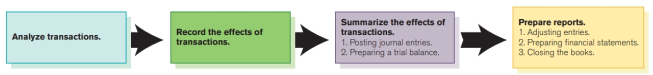
\includegraphics[width=\linewidth]{image/acc_cycle.png}
\end{figure}
%

\begin{multicols}{2}
	\begin{table}[H]
		\resizebox{\columnwidth}{!}{
			\begin{tabular}{c|c|c|c|ccc}
				& \multirow{2}{*}{Assets}  & \multirow{4}{*}{=} & \multirow{2}{*}{Liabilities} & \multicolumn{3}{c}{Equity}                             \\ \cline{5-7}
				&                &              &                 & \multicolumn{1}{c|}{Revenues} & \multicolumn{1}{c|}{Expenses} & Dividends \\ \cline{1-2} \cline{4-7}
				$\uparrow$& Dr.                  &                   &   Cr.                & Cr.                      &  Dr.                     & Dr. \\ \cline{1-2} \cline{4-7}
				$\downarrow$ &  Cr.                 &               &             Dr.      &   Dr.            &    Cr.                   & Cr.
			\end{tabular}
		}
	\end{table}
\section{Adjusting Accounts}
\textbf{Accrual Accounting} can capture the value of the firm much better due to timeliness\\
Adjusting entries made at the end of a period do not involve cash\\
Each adjusting entry involves a balance sheet account and an account on the IS/SCI;
\begin{itemize}
	\item \textbf{Unrecorded Receivables}: Amount that has not been paid but the work has been done/should be recognized (\eg billing every 3 months)
	\item \textbf{Unrecorded Liabilities}: Expenses being incurred prior to being paid or recorded (\eg interest payable, wages payable) in other words parts of expense is actually incurred due to the use of resources but it has not been paid
	\item \textbf{Prepaid Assets}: Payments that a company makes in advance for items charged to expense (\eg insurance premium payment) and the asset slowly loses its value
	\item \textbf{Unearned Revenues}: Amounts received before the actual recognition of revenues, and work is slowly being done over time which decreases liability and increases revenue
\end{itemize}
% Please add the following required packages to your document preamble:
% \usepackage{multirow}
\textbf{Accumulated Depreciation}: is a \textit{Contra-asset} with normal balance of credit
\begin{itemize}
	\item Note that for depreciation of PPE, PPE balance is not directly credited but instead Accumulated depreciation is credited (Less)
\end{itemize}
\textbf{Allowance for bad debt}: contra-asset for accounts receivable
\begin{table}[H]
	\resizebox{\columnwidth}{!}{
		\begin{tabular}{c|c|c|c|ccc}
			\multirow{2}{*}{} & \multirow{2}{*}{Assets} & \multirow{6}{*}{=} & \multirow{2}{*}{Liabilities} & \multicolumn{3}{c}{Equity}                             \\ \cline{5-7}
			&                   &                   &                   & \multicolumn{1}{c|}{Rev.} & \multicolumn{1}{c|}{Exp.} & Div.  \\ \cline{1-2} \cline{4-7}
			\makecell{Unrecorded \\Receivables}&  Dr.&  &  & Cr. &  &  \\ \cline{1-2} \cline{4-7}
			\makecell{Unrecorded \\Liabilities}&  &  & Cr. &  & Dr. &  \\ \cline{1-2} \cline{4-7}
			\makecell{Prepaid\\Expenses}&  Cr.&  &  &  & Dr. &  \\ \cline{1-2} \cline{4-7}
			\makecell{Unearned\\Revenues}&  &  & Dr.  & Cr. &  &
		\end{tabular}
	}
\end{table}

\textbf{Steps to preparing Financial Statements}
\begin{itemize}
	\item Adjust journal entries
	\item Adjust trial balance (book not closed yet)
	\item Prepare financial statements
	\begin{enumerate}
		\item IS $\rightarrow$ to calculate NI
		\item SCE $\rightarrow$ to calculate $\Delta$RE
		$$\text{RE}_1 + \text{NI} - \text{Dividends} = \text{RE}_2$$
		\item SFP (Classified)
	\end{enumerate}
    \item Close book
    \begin{itemize}
    	\item Transfer nominal accounts to RE
    \end{itemize}
    \item Post-closing trial balance
\end{itemize}

\section{Financial Statement Analysis (FSA)}
\textbf{General areas of FSA}:
\begin{itemize}
	\item \textbf{Liquidity and efficiency}: able to meet \underline{short term obligations} and efficiently generate revenues
	\item \textbf{Solvency}: able to meet \underline{long term obligations} and generate \underline{future} revenues
	\item \textbf{Profitability}: rewards for investors
	\item \textbf{Cash Flow}: manage cash inflow and outflow
	\item \textbf{Market Prospects}: generate positive market expectations
\end{itemize}

\subsection{Return on Assets (ROA)}
\begin{equation*}
	\begin{aligned}
		\text{ROA} &= \frac{\text{Net profit}}{\text{Avg total assets}}
		%&= \frac{\text{Net profit}}{\frac{\text{balance_{beginning}} + \text{balance_{ending}}}{2}}
	\end{aligned}
\end{equation*}
Measures \textit{profitability}
\subsection{Debt Ratio}
\begin{equation*}
	\begin{aligned}
		\text{Debt Ratio} = \frac{\text{Total Liabilities}}{\text{Total Assets}}
	\end{aligned}
\end{equation*}
Measures \textit{solvency} and financial leverage (higher financial leverage $\Rightarrow$ higher risk)
\subsection{Profit Margin/Return on Sales}
$$\text{Profit Margin} = \frac{\text{Net Profit}}{\text{Net Sales}}$$
\textit{Profitability?}: How much profit is generated every one dollar of sales?
\begin{itemize}
	\item Measures future growth of the company
	\item Start-ups will usually have negative growth, but if it's decreasing in magnitude it's good
\end{itemize}

\section{Exam stuff}
\begin{itemize}
	\item Record transactions: prepare journal entries
	\item prepare ledger: draw T-accounts
	\item on credit = on account
	\item Property Plant and Equipment: it's very broad and if we want to record in journal entry usually need specific accounts
	\item Write "not included in journal" when there's no exchange of goods/cash
\end{itemize}
\end{multicols}











\end{document}